\documentclass[review]{elsarticle}

\usepackage{lineno,hyperref,amsmath,siunitx}
\modulolinenumbers[5]

\journal{International Journal of Heat and Fluid Flow}

%%%%%%%%%%%%%%%%%%%%%%%
%% Elsevier bibliography styles
%%%%%%%%%%%%%%%%%%%%%%%
%% To change the style, put a % in front of the second line of the current style and
%% remove the % from the second line of the style you would like to use.
%%%%%%%%%%%%%%%%%%%%%%%

%% Numbered
%\bibliographystyle{model1-num-names}

%% Numbered without titles
%\bibliographystyle{model1a-num-names}

%% Harvard
%\bibliographystyle{model2-names.bst}\biboptions{authoryear}

%% Vancouver numbered
%\usepackage{numcompress}\bibliographystyle{model3-num-names}

%% Vancouver name/year
%\usepackage{numcompress}\bibliographystyle{model4-names}\biboptions{authoryear}

%% APA style
%\bibliographystyle{model5-names}\biboptions{authoryear}

%% AMA style
%\usepackage{numcompress}\bibliographystyle{model6-num-names}

%% `Elsevier LaTeX' style
\bibliographystyle{elsarticle-num}
%%%%%%%%%%%%%%%%%%%%%%%

\newcommand{\gqcite}{Galantucci and Quadrio \cite{galantucci2010very}}
\newcommand{\epst}{\varepsilon_\theta}

\begin{document}

\begin{frontmatter}

\title{Impact of smaller scales on the scalar dissipation rate in direct numerical simulations of wall bounded flows}
%\tnotetext[mytitlenote]{Fully documented templates are available in the elsarticle package on \href{http://www.ctan.org/tex-archive/macros/latex/contrib/elsarticle}{CTAN}.}

%% Group authors per affiliation:
\author{C\'edric Flageul, Iztok Tiselj}
\address{Reactor Engineering Division, Institut Jo\v{z}ef Stefan, Ljubljana, Slovenia}

\begin{abstract}
Passive scalar dynamics in a turbulent channel flow is studied with Direct Numerical Simulation at friction Reynolds number $Re_\tau=160$ and Prandtl number $Pr=1$. The goal of the study is to assess the grid spacing requirement for an accurate estimation of various turbulent statistics, with a special focus on the scalar dissipation rate. The implemented spatial resolutions span from the resolution comparable to the similar Direct Numerical Simulations (DNS) studies in the past, to the very fine resolution implemented by \gqcite. All scalar fields are computed in parallel using a single velocity field resolved with the finest resolution, thus reducing the statistical variability. In addition, to confidently assess the grid spacing requirement, we also evaluate the statistical uncertainty. The ``standard'' resolution of the DNS studies (resolution used by Kim et al. \cite{kim1987turbulence}) is usually sufficient for predictions of first and second-order turbulence scalar field statistics. Non-negligible corrections of the fourth-order statistics, especially the scalar dissipation variance profile, are observed with enhancement of the scalar resolution from the one used in  the ``standard'' DNS studies to the resolution recommended by Vreman and Kuerten \cite{vreman2014comparison}, which is roughly two times finer in each spatial direction. Further resolution enhancements produce only marginal differences.
\end{abstract}

\begin{keyword}
Passive scalar \sep Dissipation rate \sep Anisotropy \sep Direct Numerical Simulation \sep Channel flow \sep Sampling error
\end{keyword}

\end{frontmatter}

\linenumbers

\section{Introduction}

Since the pioneering efforts of Obukhov \cite{obukhov1968structure}, Corrsin \cite{corrsin1951spectrum} and Batchelor et al. (\cite{batchelor1959small,batchelor1959small2}), passive scalars in turbulent flows have been the focus of a number of studies. As summarized in the review by Warhaft \cite{warhaft2000passive}, experiments and simulations are challenging classical descriptions of passive scalars derived from the Kolmogorov cascade phenomenology. Evidences suggest a strong coupling between large and small scales and no local isotropy at inertial and dissipation scales. They also suggest that passive scalars are associated with a stronger intermittency compared with the velocity.

Following Batchelor et al. (\cite{batchelor1959small,batchelor1959small2}), for a unit Prandtl number as herein, the smallest spatial scale for scalar mixing is the Kolmogorov scale $\eta = \left( \nu^3 / \overline{\varepsilon} \right)^{1/4}$, where $\nu$ is the dynamic viscosity and $\overline{\varepsilon}$ the mean energy dissipation rate of the turbulent kinetic energy. Similarly, the smallest time scale is the Kolmogorov time scale $\tau_\eta = \sqrt{\nu / \overline{\varepsilon}}$. As the passive scalar is intermittent, locally, structures with a spatial (temporal) span shorter than $\eta$ ($\tau_\eta$) appear in a flow. Suspecting those fine structures to be related to highly dissipative events, a number of DNS have been performed with sub-Kolmogorov scales resolved (Schumacher et al. \cite{schumacher2005very}, Donzis and Yeung \cite{donzis2010resolution}, \gqcite).

One of the central quantity in those studies is $\epst$, the scalar dissipation rate, defined by 
\begin{equation}
\epst = 2 \alpha \lvert \nabla \theta \rvert^2 = 2 \alpha \left[ \sum_{i=1}^{3} \left( \partial_i \theta \right)^2 \right]
\end{equation}
where $\alpha$ is the thermal diffusivity. According to Pope \cite{pope2013small}, this quantity he calls the “all-important dissipation rate” matters in combustion models. It is also a central quantity in Reynolds Averaged Navier-Stokes (RANS) turbulence models as it appears in the budget equation of the scalar variance. Lately, Flageul et al. \cite{flageul2017discontinuity} showed that the dissipation rate associated with the temperature variance is discontinuous at the fluid-solid interface in case of conjugate heat transfer. This is prominent for industrial applications where thermal fatigue is a concern.

Studying homogeneous isotropic turbulence, Schumacher et al. \cite{schumacher2005very} showed that the improved resolution matters when investigating the tails of the Probability Density Function (PDF) of $\epst$, which correspond to low probability events associated with high or low dissipation rates. More specifically, they show that a poorer resolution has a stronger impact on regions of low $\epst$ than on those of high $\epst$. On a similar configuration, Donzis and Yeung \cite{donzis2010resolution} showed accurate estimation of advanced statistics (scalar dissipation intermittency exponent, structure functions at moderately high orders and PDF of $\epst$ up to 200 $\overline{\epst}$) with a grid spacing equal to the Batchelor scale, which is exactly the Kolmogorov scale in the present study.

Studying a turbulent channel flow ($Re_\tau=160$, $Pr=1$), \gqcite ~ extended the analysis to wall-bounded flows. They showed resolution effects on the profiles of the mean $\epst$ and its variance, but also on the PDF of $\epst$ and recommended a very fine spatial resolution ($\Delta_x^+=\Delta_z^+=1$ and $0.43<\Delta_y^+<2$). In the streamwise (spanwise) direction, this is 6 (4) times finer than what is necessary for the velocity according to Vreman and Kuerten \cite{vreman2014comparison}. The authors of the present study estimate that the resolution proposed by Vreman and Kuerten is sufficient for accurate predictions of the key turbulent statistics of the passive scalar field at $Pr=1$, including the average scalar dissipation rate and its variance.
 
The structure of the paper is as follows. In the second section, the governing equations and the computational setup are described alongside with the procedure to estimate the sampling error. In the third section, preliminary investigation on coarser grids is presented. In the fourth section, the DNS results are presented. Discussion and conclusions are collected in the last section.

\section{Governing equations, computational setup and sampling error}

Dimensionless equations of the incompressible turbulent channel flow with transport of a passive scalar can be found in various sources (Kasagi et al. \cite{kasagi1991direct}, Kawamura et al. \cite{kawamura1998dns}):

\begin{align}
\nabla . u & = 0 \label{eq-continuity} \\
\partial_t u & = - \nabla . \left( u . u \right) + \frac{1}{Re_\tau} \nabla^2 u - \nabla \left( p \right) + \overrightarrow{1_x} \label{eq-momentum} \\
\partial_t \theta & = - \nabla . \left( u . \theta \right) + \frac{1}{Re_\tau Pr} \nabla^2 \theta \label{eq-temperature}
\end{align}

Equations \eqref{eq-momentum} and \eqref{eq-temperature} are normalized with the channel half width $h$, the kinematic viscosity $\nu$ and the friction velocity $u_\tau$. Low friction Reynolds number $Re_\tau=160$ and Prandtl number $Pr=1$ were selected in order to replicate the conditions of the simulations performed by \gqcite. As the Prandtl number is unity, Kolmogorov and Batchelor length-scales are identical.

Periodic boundary conditions are used in the streamwise and spanwise directions, labelled $x$ and $z$, respectively, while the wall-normal direction is labelled $y$. The unit forcing term $\overrightarrow{1_x}$ is present only in the streamwise direction. Boundary conditions for the passive scalar fields at the channel walls are $\theta=1$ at $y=1$, and $\theta=-1$ at $y=-1$ and were previously used in the simulations of Papavassiliou and Hanratty \cite{papavassiliou1997transport}, Johansson and Wikstr{\"o}m \cite{johansson2000dns}, and \gqcite.

The equations are solved with a pseudo-spectral scheme. Fourier series are used in the $x$ and $z$ directions and Chebyshev polynomials are used in the $y$ direction. Second-order accurate time differencing (Crank-Nicolson scheme for diffusive terms and Adams-Bashforth scheme for other terms) is used with maximum Courant number kept at approximately $0.1$. The aliasing error is removed with computation of the nonlinear terms on a grid $1.5$ times finer in all directions. The computer code is based on the code developed by Gavrilakis et al. \cite{gavrilakis1986direct}, which was later modified by Lam and Banerjee \cite{lam1988investigation}. The code was used and verified in simulations of Tiselj et al. (\cite{tiselj2001effect}, \cite{tiselj2012dns}, \cite{tiselj2014tracking}).

The extension of the computational domain was taken from the work of \gqcite: $L_x=4.19$, $L_y=2$, and $L_z=2.09$. Such a small computational domain neglects an important part of the large scale structures in the turbulent flow, however, it is known to be sufficient for special studies focused on small scale turbulent structures of the velocity field (Jimenez and Moin \cite{jimenez1991minimal}). The small domain offers a platform for simplified studies of the resolution requirements. It is often overlooked that in addition to obliterating large scale structures, small domain can be affected by a significant sampling error. For instance, \gqcite ~ report up to $5\%$ differences in the friction temperature values in their simulations performed on different resolutions and averaged over the time interval of $2400$ viscous time units (statistics based on $60$ instantaneous fields).

\begin{table}
\begin{center}
\begin{tabular}{|c|c|c|c|c|}
\hline
Scalar field & $Nx*Ny*Nz$ & $\Delta_x^+$ & $\left[{\Delta_y^+}_{,min},{\Delta_y^+}_{,max}\right]$ & $\Delta_z^+$ \\
\hline 1KMM & $40*129*60$ & $16.8$ & $\left[0.048,3.93\right]$ & $5.57$ \\
\hline 2GQC & $64*129*64$ & $10.5$ & $\left[0.048,3.93\right]$ & $5.23$ \\
\hline 3S  & $112*129*80$ & $5.99$ & $\left[0.048,3.93\right]$ & $4.18$ \\
\hline 4VK & $112*181*80$ & $5.99$ & $\left[0.024,2.78\right]$ & $4.18$ \\
\hline 5GQM & $360*129*180$ & $1.86$ & $\left[0.048,3.93\right]$ & $1.86$ \\
\hline 6S & $360*181*180$ & $1.86$ & $\left[0.024,2.78\right]$ & $1.86$ \\
\hline
\end{tabular}
\caption{Spatial resolution for the transported passive scalar fields.}
\label{tb-resolution}
\end{center}
\end{table}

In the present study, the resolution requirement for the passive scalar field is examined with a single DNS run. The velocity field is calculated on the finest grid of $Nx*Ny*Nz = 360*181*180$ modes (Case 6S in Table \ref{tb-resolution}). Six distinct passive scalar fields are transported by this velocity field and resolved with different number of modes, see Table \ref{tb-resolution}. For the five scalar fields resolved with a lower resolution, all Fourier and Chebyshev modes above the indicated resolution are set to zero at the end of each time step.

This approach reduces the statistical variability and eases the separation of the sampling error from the error induced by a coarser spatial resolution. The separation of statistical uncertainty and resolution effects is of particular importance for the present work: the smaller extension of the domain in the homogeneous directions increases the sampling error, which easily exceeds the tiny differences induced by the variable resolution of the passive scalar field, except for simulations with a very long duration.

The finer resolution (case 6S in Table \ref{tb-resolution}) used in the wall-normal direction follows Vreman and Kuerten \cite{vreman2014comparison}. In the streamwise and spanwise directions, case 6S corresponds to the resolution used by \gqcite ~ in their ``Medium'' simulation. This is $2$ to $3$ times finer than the recommendation of Vreman and Kuerten \cite{vreman2014comparison}. Cases 5GQM and 2GQC correspond to the ``Medium'' and ``Coarse'' cases in \gqcite, respectively. The case 4VK is using the resolution recommended by Vreman and Kuerten \cite{vreman2014comparison}. The case 3S is similar to 4VK except that it uses a coarser wall-normal grid. Lastly, the resolution in case 1KMM is comparable with most of the previous DNS simulations (Kim et. al. \cite{kim1987turbulence}, Kasagi et al. \cite{kasagi1991direct}, Tiselj et al. \cite{tiselj2001effect}).

The present DNS is performed with a time step of $0.008 ~ \nu / u_\tau^2$ and one snapshot is taken every $\num{1 000}$ time steps. $700$ snapshots are used to reconstruct the statistics, corresponding to an averaging time of $\num{5 600} ~ \nu / u_\tau^2$.

DNS is widely used to produce reference data. However, as pointed out by Oliver et al. \cite{oliver2014estimating}, statistics obtained from DNS contain non-trivial errors. Errors arise mainly from the discretization of the equations and from the finite statistical sampling. As our code is based on a pseudo-spectral method and we use a fine grid, the spatial discretization error of the Navier-Stokes equation is rather low. Thus, the main source of error in our statistics is the sampling error, which we estimate with the open-source library \texttt{ar} (\url{https://github.com/RhysU/ar}, see Oliver et al. \cite{oliver2014estimating}).

The program \texttt{arsel}, which ships with the library, is used as follows. For each statistical quantity of interest, the instantaneous value is extracted from each snapshot and averaged in the homogeneous directions. The resulting time series are used to fit autoregressive models with \texttt{arsel} using the \texttt{--subtract-mean} option. The output of \texttt{arsel} is then processed to extract the average profile and the sampling error profile. Herein, the sampling error is given as $2$ standard deviations. Given the domain extension, the number of modes used and the time step, the probability that the real average and its estimation differ for less than $2$ standard deviations is $95\%$.

As this method can be applied for any statistical quantity, we are able to estimate the sampling error for the mean temperature, the temperature dissipation rate or its variance. For a given variable $\phi$, the associated sampling error is $e_\phi$. We also define the dimensionless normalized sampling error $E\left[\phi\right]$ by
\begin{equation}
E\left[\phi\right]\left(y\right) = \frac{e_\phi \left(y\right)}{e_\phi \left(y\right) + \mbox{abs}\left( \overline{\phi \left(y\right)} \right)}
\end{equation}
This normalized sampling error is bounded in $[0,1]$, the upper bound being reached when the averaged value $\mbox{abs}\left( \overline{\phi \left(y\right)} \right)$ is exactly zero. As most of the time the averaged value is large compared to the sampling error, $E\left[\phi\right]$ measures the relative uncertainty.

\section{Preliminary results on coarser grids}

The sampling error on $u_\tau^2$, whose theoretical value is $1$ herein, and $\partial_y \overline{\theta} \left( y = \pm 1 \right)$ is illustrated with the four DNS studies on coarser grids described in the Table \ref{tb-coarse}. The results in the large computational box combined with the long and short averaging time are taken from the analyses of Tiselj and Cizelj \cite{tiselj2012dns}, which were performed at $Re_\tau=180$, $Pr=1$ and with slightly different thermal boundary conditions: both channel walls were heated and a forcing term was present in the passive scalar equation \eqref{eq-temperature}. The small box results are part of the present analysis: a separate run over longer time interval was made only with a resolution, which corresponds to the case 1KMM in Table \ref{tb-resolution}.

\begin{table}
\begin{center}
\begin{tabular}{|@{}c@{}|c|c|c|@{}c@{}|@{}c@{}|@{}c@{}|}
\hline
Label & $Re_\tau$ & \begin{tabular}{@{}c@{}} $L_x^+$ \\ $L_y^+$ \\ $L_z^+$ \end{tabular} & \begin{tabular}{@{}c@{}} $\Delta_x^+$ \\ ${\Delta_y^+}_{,max}$ \\ $\Delta_z^+$ \end{tabular} & \begin{tabular}{@{}c@{}} Averaging time \\ (wall units) \end{tabular} & $u_\tau^2 \pm e_{u_\tau^2}$ & $\partial_y \overline{\theta} \pm e_{\partial_y\overline{\theta}}$ \\
\hline
\begin{tabular}{c} 18L \\ \hline 18S \end{tabular} &
$180$ &
\begin{tabular}{@{}c@{}} $6786$ \\ $360$ \\ $2262$ \end{tabular} &
\begin{tabular}{@{}c@{}} $17.7$ \\ $4.42$ \\ $5.89$ \end{tabular} &
\begin{tabular}{c} \begin{tabular}{@{}c@{}} $\num{24300}$ \\ (450 samples) \end{tabular} \\ \hline
                   \begin{tabular}{@{}c@{}} $\num{5400}$ \\ (100 samples) \end{tabular} \end{tabular} &
\begin{tabular}{c} \begin{tabular}{@{}c@{}} $1.0004\pm0.0016$ \\ $0.9998\pm0.0016$ \end{tabular} \\ \hline
                   \begin{tabular}{@{}c@{}} $0.9997\pm0.0029$ \\ $1.0005\pm0.0033$ \end{tabular} \end{tabular} &
\begin{tabular}{c} \begin{tabular}{@{}c@{}} $-180.11\pm0.15$ \\ $180.01\pm0.14$ \end{tabular} \\ \hline
                   \begin{tabular}{@{}c@{}} $-179.74\pm0.29$ \\ $180.14\pm0.46$ \end{tabular} \end{tabular} \\
\hline
\begin{tabular}{c} 16L \\ \hline 16S \end{tabular} &
$160$ &
\begin{tabular}{@{}c@{}} $670$ \\ $320$ \\ $334$ \end{tabular} &
\begin{tabular}{@{}c@{}} $16.8$ \\ $3.93$ \\ $5.57$ \end{tabular} &
\begin{tabular}{c} \begin{tabular}{@{}c@{}} $\num{24000}$ \\ (500 samples) \end{tabular} \\ \hline
                   \begin{tabular}{@{}c@{}} $\num{6000}$ \\ (125 samples) \end{tabular} \end{tabular} &
\begin{tabular}{c} \begin{tabular}{@{}c@{}} $1.002\pm0.014$ \\ $1.003\pm0.019$ \end{tabular} \\ \hline
                   \begin{tabular}{@{}c@{}} $1.005\pm0.026$ \\ $0.990\pm0.050$ \end{tabular} \end{tabular} &
\begin{tabular}{c} \begin{tabular}{@{}c@{}} $6.80\pm0.05$ \\ $6.78\pm0.08$ \end{tabular} \\ \hline
                   \begin{tabular}{@{}c@{}} $6.82\pm0.10$ \\ $6.63\pm0.24$ \end{tabular} \end{tabular} \\
\hline
\end{tabular}
\end{center}
\caption{Sampling error on friction velocity and temperature derivative at the boundaries.}
\label{tb-coarse}
\end{table}

The first impression about the statistical uncertainty can be obtained from the last two columns of Table \ref{tb-coarse} where the squared friction velocities and temperature derivatives at both channel walls are shown. As one might expect, deviation from the theoretical friction velocity of $1$ is larger in the smaller computational domain and at shorter averaging time intervals. As for the temperature derivative, shorter averaging time also leads to higher sampling error. Regarding cases $Re_\tau=160$, we observe a relatively large difference on the temperature derivative at both walls. Although this difference gets lower when increasing the duration of the simulation, it is probably specific to smaller computational domains, as reported by Jimenez and Moin \cite{jimenez1991minimal} for velocity statistics.

\begin{figure}[htbp]
\begin{center}
\includegraphics[width=\textwidth]{../PLOTS/tmean.pdf}
\begin{tabular}{cc}
\includegraphics[width=0.5\textwidth]{../PLOTS/tvariance.pdf} & 
\includegraphics[width=0.5\textwidth]{../PLOTS/dissipation.pdf} \\
\includegraphics[width=0.5\textwidth]{../PLOTS/t4.pdf} & 
\includegraphics[width=0.5\textwidth]{../PLOTS/diss_variance.pdf}
\end{tabular}
\end{center}
\caption{Normalized sampling error for the cases in Table \ref{tb-coarse}. Top: $E\left[ \theta \right]$. Middle: $E\left[ \theta'^2 \right]$ (left) and $E\left[ \epst \right]$ (right). Bottom: $E\left[ \theta'^4 \right]$ (left) and $E\left[ \epst^2 \right]$ (right).}
\label{fig-coarse}
\end{figure}

The case 16S in Table \ref{tb-coarse} is comparable to the case 1KMM in Table \ref{tb-resolution}. Both cases correspond to an averaging time roughly $2$ times longer than the one in \gqcite, with snapshots taken at a similar frequency for all those cases. Thus, the case 16S gives a lower bound for the sampling error in \gqcite. The Figure \ref{fig-coarse} shows the normalized sampling error associated with various statistical quantities for the cases present in Table \ref{tb-coarse}.

The clear trend is that higher order moments are associated with higher sampling errors. Regarding the plots on the middle row, the normalized sampling error for the temperature variance and for the mean dissipation rate have a similar amplitude and involve turbulent quantities to the power $2$. Qualitatively, the situation is similar on the plots in the bottom row, which involve average of turbulent quantities to the power $4$.

Regarding case 16S, the magnitude of the normalized sampling error is around $5\%$ for $E\left[\theta\right]$, except in the middle of the channel, where it gets close to $100\%$ as the average temperature is zero. It also drops down to zero at the walls as the temperature is imposed there (Dirichlet boundary condition, $\theta = \pm 1$). For cases 18S and 18L, the imposed temperature at the walls is zero, so both the sampling error and the average temperature tend to zero there. The resulting normalized sampling error $E\left[\theta\right]$ at the wall for those cases is around $0.2\%$.

Focusing on case 16S for higher order statistics, the normalized sampling error reaches almost $10\%$ for $E\left[ \theta^{\prime2} \right]$ and $E\left[\epst\right]$, and even $15\%$ for $E\left[ \theta^{\prime4} \right]$ and $E\left[\epst^2\right]$. These results show that the differences of $7\%$ on the average of $\epst$ on different grid reported in \gqcite ~ is well within the sampling error as their simulations have the same domain extension but a duration halved compared with the case 16S.

Using the Central Limit Theorem applied to weakly correlated samples described in Oliver et al. \cite{oliver2014estimating} (Theorem 27.4 in Billingsley \cite{billingsley2008probability}), the sampling error decreases with the square root of the number of samples. For a given sampling frequency, the error is therefore halved when the duration of the simulation (and the number of samples) is increased by a factor $4$. This holds quite well when comparing cases 16S and 16L, or 18S and 18L. Overall, significant reduction of the sampling error can be achieved using extended computational domains and / or simulations with a longer duration.

\section{Impact of smaller scales on statistics}

In this section, we investigate the impact of smaller scales on various quantities. First, we investigate dimensionless bulk quantities. Using the scalar with the finest resolution (6S) as a reference, we can compute a quadratic relative error. For instance, the quadratic relative error for the average temperature on the grid 1KMM is defined by:
\begin{equation}
\frac{\int_{y=-1}^{y=1}\left[\,\overline{\theta_{1KMM}}\left(r\right) - \overline{\theta_{6S}}\left(r\right)\right]^2\mbox{dr}}{\int_{y=-1}^{y=1}{\overline{\theta_{6S}}\left(r\right)}^2\mbox{dr}}
\end{equation}

In Table \ref{tb-error}, the quadratic relative error is given for various quantities. Looking at the relative error for the moments of the temperature ($\theta$, $\theta^{\prime2}$, $\theta^{\prime3}$ and $\theta^{\prime4}$), one can extract two trends. First, for all resolutions considered, the higher the moment, the higher the relative error. Second, the finer the resolution, the closer to the case 6S. The resolution 1KMM seems sufficient to accurately estimate the average temperature. However, accurate estimation of higher order moments requires a finer resolution as smaller scales have a higher impact on them. The situation is similar for $\epst$ and $\epst^{\prime2}$: the first is relatively well estimated by the coarsest grid while the second has a stronger dependence on smaller scales.

\begin{table}
\begin{center}
\begin{tabular}{|c|c|c|c|c|c|c|c|}
\hline
Scalar field & $Nx*Ny*Nz$ & $\theta$ & $\theta'^2$ & $\theta'^3$ & $\theta'^4$ & $\epst$ & $\epst'^2$ \\
\hline
1KMM & $40*129*60$ & $-7.18$ & $-5.02$ & $-4.42$ & $-3.67$ & $-6.68$ & $-1.26$ \\
\hline
2GQC & $64*129*64$ & $-9.15$ & $-7.14$ & $-6.50$ & $-5.43$ & $-7.82$ & $-1.91$ \\
\hline
3S & $112*129*80$ & $-11.8$ & $-10.5$ & $-8.57$ & $-8.11$ & $-9.54$ & $-3.25$ \\
\hline
4VK & $112*181*80$ & $-11.8$ & $-10.5$ & $-8.58$ & $-8.13$ & $-9.98$ & $-3.29$ \\
\hline
5GQM & $360*129*180$ & $-13.9$ & $-12.0$ & $-10.0$ & $-10.8$ & $-9.51$ & $-5.53$ \\
\hline
\end{tabular}
\end{center}
\caption{$log_{10}$ of the quadratic relative error for various quantities.}
\label{tb-error}
\end{table}

It is important to stress that the discretization error in Table \ref{tb-error} is typically several decades lower than the sampling error. However, all the scalar fields are transported by the same velocity field. Therefore, they are strongly correlated and are all plagued by the same sampling error. This allows us to exhibit the impact of smaller scales on statistics, even though this impact is relatively small compared with the sampling error.

For the turbulent channel flow studied here, at the wall, the temperature is imposed ($\theta = \pm 1$) and the temperature evolution equation \ref{eq-temperature} contains no source term. As a result, the exact average temperature derivative at the wall is plagued by statistical uncertainty and depends on the spatial resolution. We define the friction temperature $\theta_\tau$ and the reference temperature $\theta_{ref}$ with:
\begin{equation}
\theta_\tau = \frac{1}{Re_\tau Pr} \partial_y \overline{\theta} \left(\pm \frac{L_y}{2} \right)
\mbox{ and }
\theta_{ref} = \frac{1}{Re_\tau Pr} \frac{\overline{\theta}\left(L_y/2\right)-\overline{\theta}\left(-L_y/2\right)}{L_y}
\end{equation}

The theoretical value of the friction velocity, which is equal to one here, produces a $\theta_{ref}$ not plagued by statistical uncertainty, while $\theta_\tau$ is. Therefore, we use $\theta_{ref}$ to rescale the temperature statistics. Spatial derivatives are expressed in wall-units using the theoretical value of the friction velocity. For convenience, plots are using a wall-normal distance in bulk units ($y \in \left[ -1,1 \right]$).

Complementary with the bulk quantities in Table \ref{tb-error} and the integral profiles of $\epst$ or its variance, we investigate the anisotropy of the fluctuating temperature gradient. This is done using the barycentric map defined by Banerjee et al. \cite{banerjee2007presentation}. Given a symmetric positive semi-definite tensor $M_{ij}$, the associated (traceless) anisotropy tensor is
\begin{equation}
\widetilde{M_{ij}} = \frac{M_{ij}}{M_{kk}}-\frac{1}{3} \delta_{i,j}
\end{equation}
The eigenvalues of $\widetilde{M_{ij}}$, $\lambda_k$, verify $\lambda_1 \geq \lambda_2 \geq \lambda_3$. Based on those eigenvalues, Banerjee et al. \cite{banerjee2007presentation} define 3 limiting states forming a basis: one-component (1C), two-component (2C) and three-component (3C). The number of components corresponds to the number of non-zero eigenvalues of $M_{ij}$. In the state 3C, all three eigenvalues are equal: the tensor is isotropic. In the state 2C, one eigenvalue is negligible while the two others are equal: the anisotropy is two-dimensional. In the state 1C, two eigenvalues are negligible: the anisotropy is one-dimensional.

In the barycentric map, each limiting state is the vertex of an equilateral triangle. For any symmetric positive semi-definite tensor $M_{ij}$, there is a unique point inside this equilateral triangle with coordinates
\begin{equation}
\left[ x,y \right] = \left( \lambda_1 - \lambda_2 \right) \left[ x_{1C},y_{1C} \right] + 2 \left( \lambda_2 - \lambda_3 \right) \left[ x_{2C},y_{2C} \right] + \left( 3\lambda_3 + 1 \right) \left[ x_{3C},y_{3C} \right]
\end{equation}
where $\left[x_{iC},y_{iC} \right]$ is the coordinate of the vertex corresponding to the limiting state iC. Following Lumley and Newman \cite{lumley1977return}, it is possible to visualize the anisotropy of a traceless tensor using its second and third invariants. However, the resulting invariant map is distorted as those invariants are nonlinear functions of the tensor’s elements. The barycentric map is connected to the invariant map with a bijection and does not suffer from this bias. This is the main motivation for the present choice; interested reader will find a deeper analysis of the barycentric map in Banerjee et al. \citep{banerjee2007presentation}.

The symmetric positive semi-definite tensors investigated here are related to the temperature derivatives. The first tensor investigated, $\overline{\overline{\partial \theta}} = \overline{\partial_i \theta' \partial_j \theta' }$, is relevant to this study as its trace is proportional to the scalar dissipation rate εθ and its anisotropy is related to the anisotropy of the fluctuating temperature gradient. The other tensor investigated is the variance of $\overline{\overline{\partial \theta}}$ : $\sigma_{\overline{\overline{\partial \theta}}} = \overline{\left[\partial_i \theta' \partial_j \theta' \right]^2 } - \left[ \, \overline{\partial_i \theta' \partial_j \theta' } \, \right]^2$. Locations where the fluctuating temperature gradient is isotropic correspond to points of the barycentric map closer to the vertex 3C of the triangle. The further away from this vertex, the higher the anisotropy. Points closer to 1C or 2C correspond to one-dimensional or two-dimensional fluctuations, respectively. It is important to stress that the barycentric map does not provide a complete description of the anisotropy as it obliterates the eigenvectors associated with the eigenvalues.

\begin{figure}[htbp]
\begin{center}
\begin{tabular}{cc}
\includegraphics[width=0.5\textwidth]{../data/diss.pdf} & 
\includegraphics[width=0.5\textwidth]{../data/dissa.pdf}
\end{tabular}
\end{center}
\caption{Dissipation rate $\overline{\epst}$ (left) and barycentric map associated with $\overline{\overline{\partial \theta}}$ (right).}
\label{fig-diss}
\end{figure}

The Figure \ref{fig-diss} left is in agreement with Table \ref{tb-error}; the profiles of $\epst$ do not show any significant impact of unresolved smaller scales in 1KMM and 3S results. The situation is similar for the barycentric map of the anisotropy of $\overline{\overline{\partial \theta}}$ (Figure \ref{fig-diss} right). Due to the imposed temperature at the wall, the anisotropy at the boundary has only one component (limiting state 1C). Then, the closer to the middle of the channel, the closer to isotropy (limiting state 3C).

\begin{figure}[htbp]
\begin{center}
\begin{tabular}{cc}
\includegraphics[width=0.5\textwidth]{../data/var_diss.pdf} & 
\includegraphics[width=0.5\textwidth]{../data/var_dissa.pdf}
\end{tabular}
\end{center}
\caption{$95 \%$ confidence interval of the variance of the dissipation rate $\epst$ (left) and barycentric map associated with $\sigma_{\overline{\overline{\partial \theta}}}$ (right).}
\label{fig-var_diss}
\end{figure}

Figure \ref{fig-var_diss} left is also in agreement with Table \ref{tb-error}; the variance of $\epst$ is significantly impacted by smaller scales, and the coarsest grid underestimates this quantity, especially outside of the viscous sublayer where the discretization error is as large as the sampling error. Closer to the wall, this impact is less visible and all spatial resolutions produce a similar variance of $\epst$. The barycentric map of the anisotropy of $\sigma_{\overline{\overline{\partial \theta}}}$ also shows the impact of smaller scales. In the middle of the channel, the coarsest grid gives a similar weighting for all limiting states (1C, 2C and 3C), this correspond to the part of 1KMM closer to the middle of the triangle. At this location of the channel, finer grids give a similar weighting only for the limiting states 1C and 3C, but a negligible weight to state 2C, this correspond to the part of 6S and 3S closer to the edge connecting 1C and 3C.

\begin{figure}[htbp]
\begin{center}
\begin{tabular}{cc}
\includegraphics[width=0.5\textwidth]{../data/x4.pdf} & 
\includegraphics[width=0.5\textwidth]{../data/z4.pdf}
\end{tabular}
\end{center}
\caption{Spectra of the streamwise (left) and spanwise (right) contributions to the scalar dissipation rate $\epst$ at $y=0$ (middle of the channel).}
\label{fig-spec}
\end{figure}

Integral quantities provide only a limited amount of information and spectra in Figure \ref{fig-spec} are more insightful. They are taken at the middle of the channel ($y=0$). The spanwise spectra show that the spanwise contribution to $\epst$ is well resolved even on the coarsest grid. However, this grid is not isotropic and it has extended cells in the streamwise direction ($\Delta_x^+=17$, $\Delta_z^+=6$ for 1KMM). This leads to a pronounced bump on the streamwise spectrum of 1KMM at the highest resolved wavenumbers ($k_x^+\approx 20$). As one can notice, the streamwise spectrum of 3S also has a bump at the highest resolved frequency ($k_x^+\approx 55$). However, regarding the latter case, this has a negligible impact on the statistics of $\epst$ because the bumps correspond to very high frequencies for which the streamwise contribution to the dissipation is two decades smaller than its peak value around $k_x^+ \approx 0.05$. This does not hold for case 1KMM: the bump on the streamwise spectrum is present at lower frequencies, for which the streamwise contribution to the dissipation has a magnitude similar to the one at the peak. This explains the severe impact of smaller scales on the variance of $\epst$ exhibited in  Figure \ref{fig-var_diss}.

\begin{figure}[htbp]
\begin{center}
\begin{tabular}{cc}
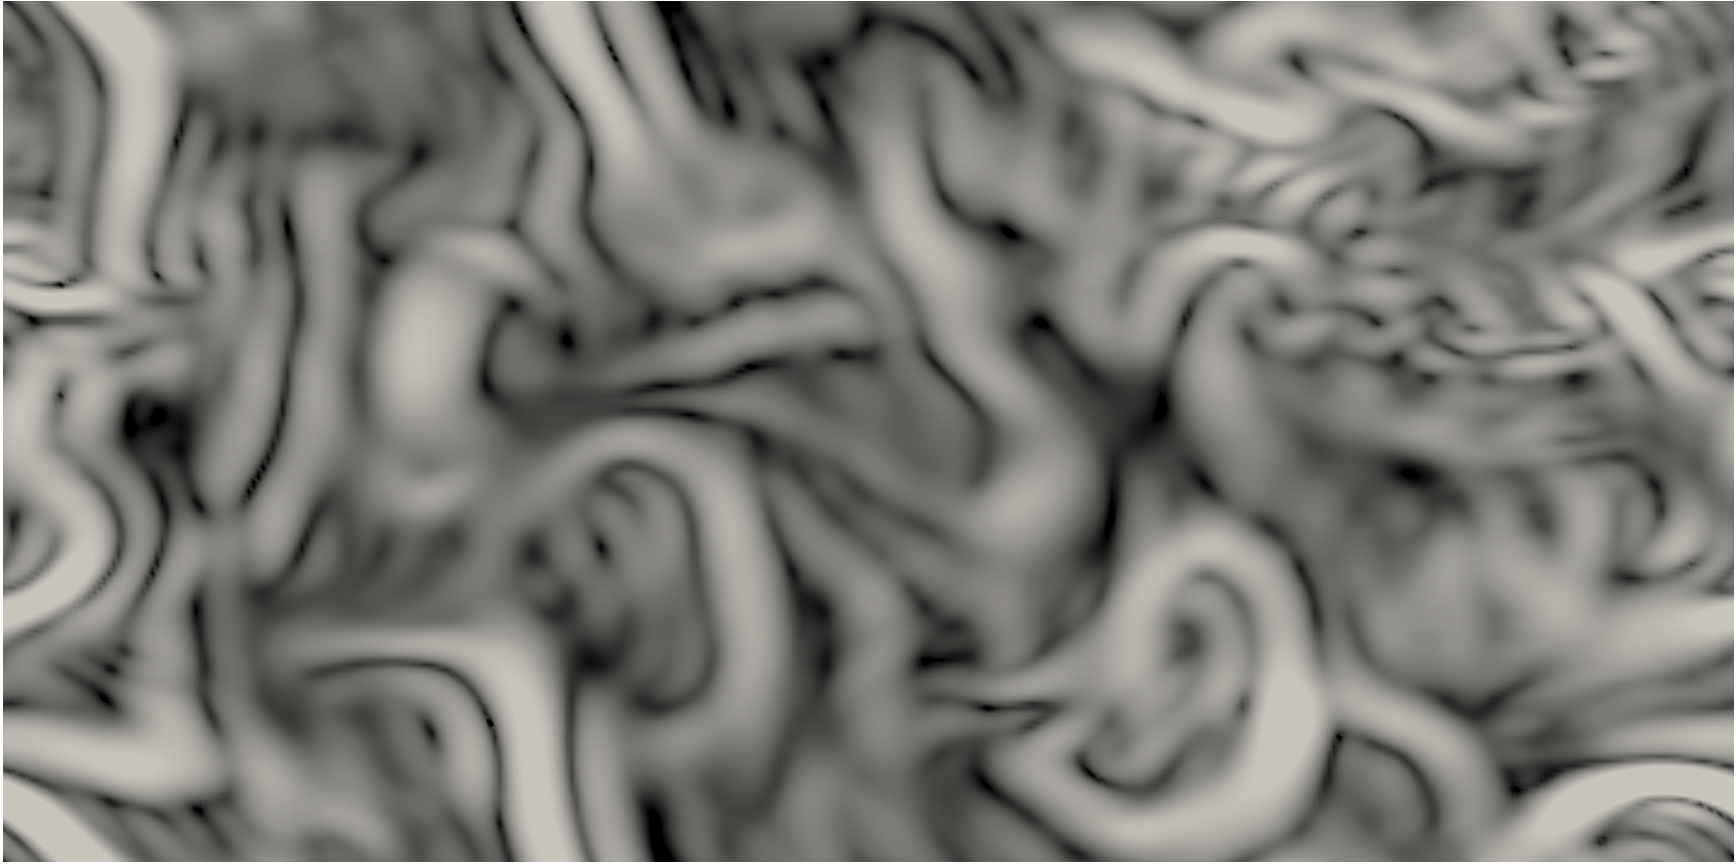
\includegraphics[width=0.5\textwidth]{../visu/diss1KMM.png} & 
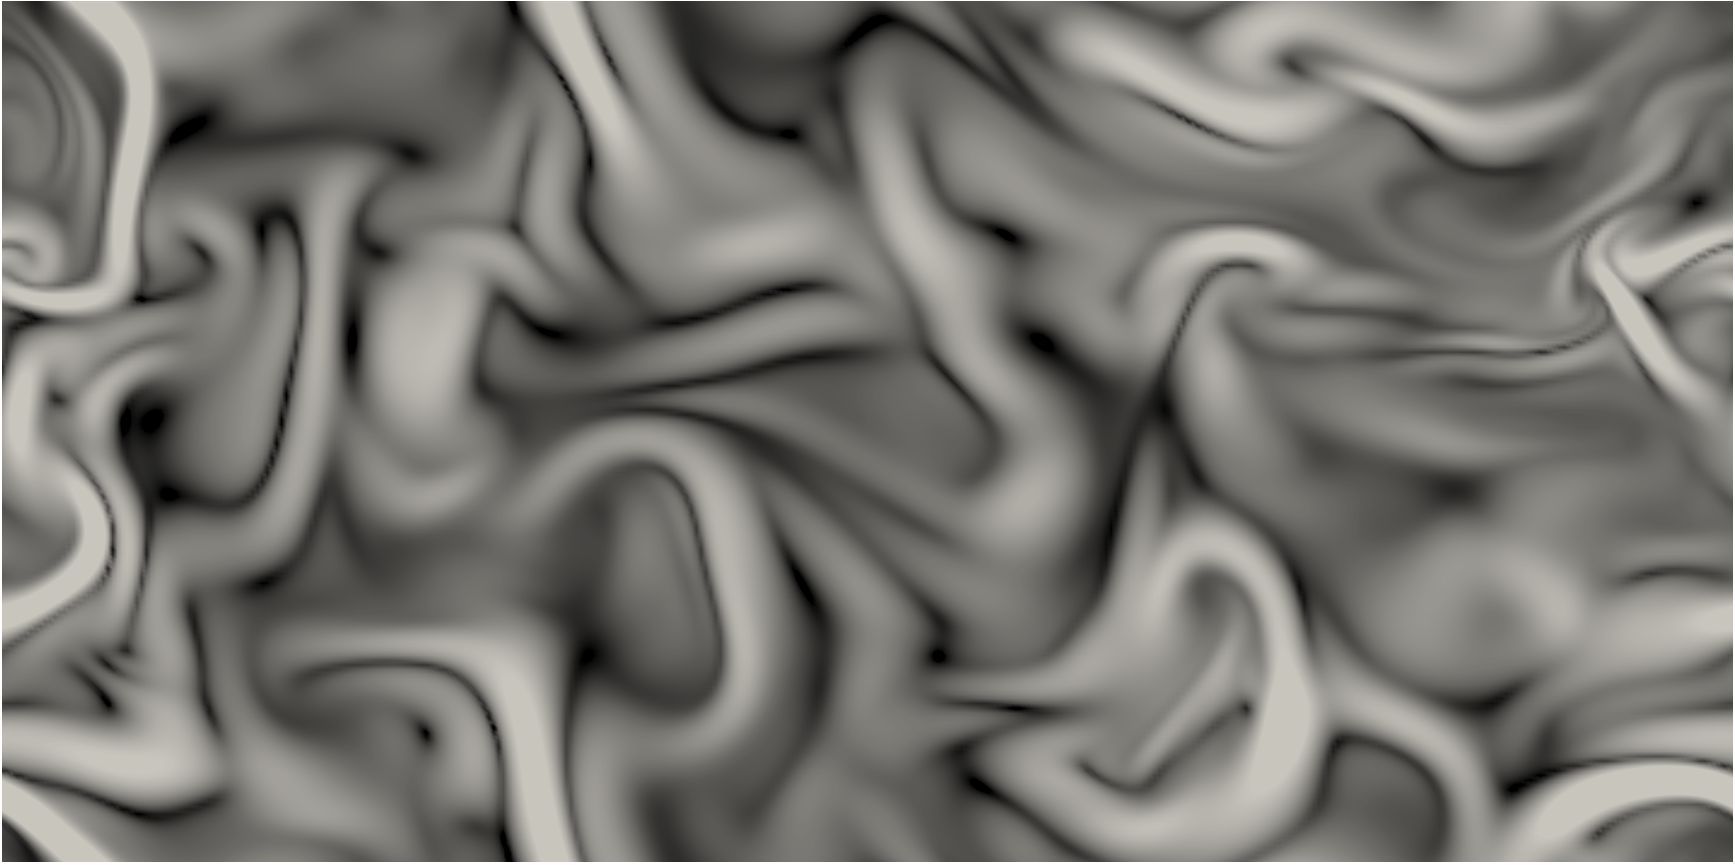
\includegraphics[width=0.5\textwidth]{../visu/diss6S.png}
\end{tabular}
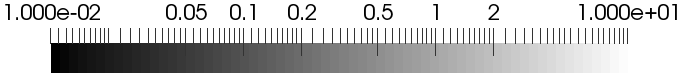
\includegraphics[width=\textwidth]{../visu/diss_colorbar.png}
\end{center}
\caption{Instantaneous scalar gradient ($\sum \partial_i \theta^{\prime 2}$) in bulk units at $y=0$ (middle of the channel). Logarithmic colormap. Left: 1KMM. Right: 6S.}
\label{fig-visu}
\end{figure}

Figure \ref{fig-visu} illustrates the impact of the under-resolution on the gradient of the scalar. On the one hand, both fields exhibit similar structures at larger scales, in agreement with the ability of the grid 1KMM to estimate the average dissipation rate, as shown in Figure 2. On the other hand, smaller scales are visibly misrepresented on the coarser grid, as the picture on the left is plagued by the oscillations, which correspond to the wavenumbers of around $k^+=20$ that are overpredicted in 1KMM results shown in Figure \ref{fig-spec} left. This is consistent with the previous results: the grid 1KMM is too coarse to properly resolve the sharp gradients which separates dissipative and non-dissipative regions.

\section{Conclusion}

The present investigation demonstrates the impact of smaller scales on the scalar dissipation rate, its variance and on the anisotropy of the fluctuating scalar gradient. In a preliminary part, we showed that simulations of the turbulent channel flow based on smaller domains and with a limited duration (often used to perform grid sensitivity analysis) are plagued by a relatively large sampling error, especially for higher order moments like the scalar dissipation rate or its variance. This sampling error is often larger than the discretization error, thus preventing accurate estimation of the latter, except for simulations with an extended domain and duration.

This situation is overcome when using a single velocity field to transport several passive scalars with different resolutions: all the scalars are strongly coupled by the velocity field and plagued by the same sampling error. The resulting difference between the scalars is solely due to the discretization error, which can thus be estimated.

Our results demonstrate that previous DNS based on a pseudo-spectral method with the resolution 1KMM (Kim et. al. \cite{kim1987turbulence}, Kasagi et al. \cite{kasagi1991direct}, Tiselj et al. \cite{tiselj2001effect}) can estimate the average temperature, its variance and the average scalar dissipation rate with a relatively low discretization error, as indicated Table \ref{tb-error}. However, they can only provide qualitative estimation for higher order moments. To accurately estimate those higher order moments, finer grids must be used. Regarding the variance of the scalar dissipation rate, or the anisotropy of the fluctuating scalar gradient, the grid recommended by Vreman and Kuerten \cite{vreman2014comparison} is sufficient for pseudo-spectral schemes (finite-difference schemes require a grid 4/3 finer). Our results do not preclude existence of scalar structures or events, which are too small to be resolved with the Vreman and Kuerten resolution. However, our results show that these events might affect only the turbulence statistics higher than fourth-order.

Our results also demonstrate that smaller scales have a stronger impact outside of the viscous sublayer, and have almost no impact closer to the wall. Strictly speaking, this observation is valid only for the Dirichlet boundary condition investigated here (imposed temperature), and may not hold for a Neumann boundary condition (imposed heat flux), a Robin boundary condition (heat exchange coefficient) or conjugate heat-transfer (fluid-solid thermal coupling). Regarding the latter case, the present analysis will provide a solid ground for future investigations on the discontinuity of $\epst$ at the fluid-solid interface.

Data associated with the present paper are available online at \url{http://dx.doi.org/10.17632/mn74gv69wn.1} and \url{https://repo.ijs.si/CFLAG/sml-scl} under the GNU GPL v3 licence.

\section*{Acknowledgements}

This work was financially supported by the research project of the Slovenian Research Agency P2-0026 and by the EDF-JSI collaboration, project PR-07184.

\section*{References}

\bibliography{mybibfile}

\end{document}
